\documentclass{lecture}

\institute{Institut für Statistik und Wirtschaftsmathematik}
\title{Vorlesung 1}
\author{Joshua Feld, 406718}
\course{Statistik}
\professor{Cramer}
\semester{Sommersemester 2022}
\program{CES (Bachelor)}

\begin{document}
    \maketitle


    \section*{Einführung und Grundbegriffe}

    Zu den Themen der angewandten Statistik gehören die Erhebung von Daten, deren Aufbereitung, Beschreibung und Analyse.
    Unter Nutzung der Werkzeuge der Beschreibenden (oder Deskriptiven) Statistik ist das Entdecken von Strukturen und Zusammenhängen in Datenmaterial ein wichtiger Aspekt der Statistik, die in diesem Verständnis auch als explorative Datenanalyse bezeichnet wird.
    Um ein methodisches Instrumentarium zur Bearbeitung dieser Aufgaben entwickeln zu können, ist es notwendig, von konkreten Einzelfällen zu abstrahieren und allgemeine Begriffe für die Aspekte, die im Rahmen einer statistischen Untersuchung von Interesse sind, bereitzustellen.

    Zunächst ist zu spezifizieren, über welche Gruppe von Personen (z.B. Schülerinnen, Schüller, Studierende oder Berufstätige) oder Untersuchungseinheiten (z.B. Geräte oder Betriebe) welche Informationen gewonnen werden sollen.
    Besteht Klarheit über diese grundlegenden Punkte, so ist festzuhalten, wie die Studie durchgeführt wird.
    Häufig werden nicht alle Elemente (statistische Einheiten) der spezifizierten Menge (Grundgesamtheit) betrachtet, sondern in der Regel wird lediglich eine Teilgruppe (Stichprobe) untersucht.
    An den Elementen dieser Stichprobe werden dann die für die statistische Untersuchung relevanten Größen (Merkmale) gemessen.
    Die resultierenden Messergebnisse (Daten) ermöglichen den Einsatz statistischer Methoden, um Antworten auf die zu untersuchenden Fragestellungen zu erhalten.
    Im Folgenden werden die genannten Begriffe näher erläutert.


    \section*{Grundgesamtheit und Stichprobe}

    In jeder statistischen Untersuchung werden Daten über eine bestimmte Menge einzelner Objekte ermittelt.
    Diese Menge von räumlich und zeitlich eindeutig definierten Objekten, die hinsichtlich bestimmter -- vom Ziel der Untersuchung abhängender -- Kriterien übereinstimmen, wird als Grundgesamtheit bezeichnet.
    Eine andere, häufig anzutreffende Bezeichnung ist Population.

    \begin{example}
        Wird eine Untersuchung über die Grundfinanzierung der Studierenden in einem bestimmten Sommersemester gewünscht, so legt die Gesamtheit aller Studierenden, die in dem betreffenden Semester immatrikuliert sind, die Grundgesamtheit fest.
        Ehe die Untersuchung begonnen werden kann, sind natürlich noch eine Reihe von Detailfragen zu klären:
        welche Hochschulen werden in die Untersuchung einbezogen, welchen Status sollen die Studierenden haben (Einschränkung auf spezielle Semester, Gasthörer/innen, \(\ldots\)) etc.
    \end{example}

    In der Praxis können Probleme bei der exakten Beschreibung einer für das Untersuchungsziel relevanten Grundgesamtheit auftreten.
    Eine eindeutige Beschreibung und genaue Abgrenzung ist jedoch von besonderer Bedeutung, um korrekte statistische Aussagen ableiten und erhaltene Ergebnisse interpretieren zu können.

    \begin{example}
        In einer statistischen Untersuchung sollen Daten über die Unternehmen eines Bundeslands erhoben werden.
        Hierzu muss geklärt werden, ob unterschiedliche Teile eines Unternehmens (wie z.B. Lager oder Produktionsstätten), die an verschiedenen Orten angesiedelt sind, jeweils als einzelne Betriebe gelten oder ob lediglich das gesamte Unternehmen betrachtet wird.
        Es ist klar, dass sich abhängig von der Vorgehensweise eventuell völlig unterschiedliche Daten ergeben.
    \end{example}

    Die Elemente der Grundgesamtheit werden als statistische Einheiten bezeichnet.
    Statistische Einheiten sind also diejenigen Personen oder Objekte, deren Eigenschaften für eine bestimmte Untersuchung von Interesse sind.
    Alternativ sind auch die Bezeichnungen Merkmalsträger, Untersuchungseinheit oder Messobjekt gebräuchlich.

    \begin{example}
        \begin{enumerate}
            \item An einer Universität wird eine Erhebung über die Ausgaben der Studierenden für Miete, Kleidung und Freizeitgestaltung durchgeführt.
            Die statistischen Einheiten in dieser Untersuchung sind die Studierenden der Universität.
            Die genannten Ausgaben sind die für die Analyse relevanten Eigenschaften.
            \item In einem Bundesland werden im Rahmen einer statistischen Untersuchung die Umsätze von Handwerksbetrieben analysiert.
            Die Handwerksbetriebe des Bundeslands sind in diesem Fall die statistischen Einheiten.
            Die in jedem Betriebs auszuwertende Größe ist der Umsatz.
        \end{enumerate}
    \end{example}

    Ziel jeder statistischen Untersuchung ist es, anhand von Daten Aussagen über eine Grundgesamtheit zu treffen.
    Aus praktischen Erwägungen kann in der Regel jedoch nicht jede statistische Einheit der Grundgesamtheit zur Ermittlung von Daten herangezogen werden.
    Ein solches Vorgehen wäre häufig zu zeit- und kostenintensiv.
    Im Extremfall ist es sogar möglich, dass durch den Messvorgang die zu untersuchenden Objekte unbrauchbar werden (z.B. bei Lebensdauertests von Geräten oder der Zugfestigkeit eines Stahls).
    In diesem Fall ist es offenbar nicht sinnvoll, eine Messung an allen zur Verfügung stehenden Objekten durchzuführen.

    \begin{example}
        Bei einer Volkszählung werden Daten über die gesamte Bevölkerung eines Landes durch Befragung jeder Einzelperson ermittelt.
        Da die Durchführung einer vollständigen Volkszählung mit hohem zeitlichem und personellem Aufwand verbunden und daher kostenintensiv ist, wird diese nur sehr selten realisiert.
        Um trotzdem eine Fortschreibung der gesellschaftlichen Veränderungen zu ermöglichen, werden regelmäßig Teilerhebungen vom Statistischen Bundesamt Deutschland durchgeführt.
        Beim so genannten Mikrozensus wird jährlich \(1\%\) der in Deutschland lebenden Bevölkerung hinsichtlich verschiedener Größen befragt (z.B. Erwerbsverhalten, Ausbildung, soziale und familiäre Lage).
    \end{example}

    Aus den genannten Gründen werden Daten oft nur für eine Teilmenge der Objekte der Grundgesamtheit ermittelt.
    Eine solche Teilmenge wird als Stichprobe bezeichnet.
    Aufgrund des geringeren Umfangs ist die Erhebung einer Stichprobe im Allgemeinen kostengünstiger als eine vollständige Untersuchung aller Objekte.
    Insbesondere ist die Auswertung des Datenmaterials mit geringerem Zeitaufwand verbunden.
    Um zu garantieren, dass die Verteilung der zu untersuchenden Eigenschaften (Merkmalsausprägungen) der statistischen Einheiten in der Stichprobe mit deren Verteilung in der Grundgesamtheit annähernd übereinstimmt, werden die Elemente der Stichprobe häufig durch zufallsgesteuerte Verfahren ausgewählt.
    Solche Verfahren stellen sicher, dass prinzipiell jeder Merkmalsträger der Grundgesamtheit mit derselben Wahrscheinlichkeit in die Stichprobe aufgenommen werden kann (Zufallsstichprobe).
    Die Auswahl einer Stichprobe wird in dieser Vorlesung nicht behandelt.


    \section*{Merkmale und Merkmalsausprägungen}

    Eine spezielle Eigenschaft statistischer Einheiten, die im Hinblick auf das Ziel einer konkreten statistischen Untersuchung von Interesse ist, wird als Merkmal bezeichnet.
    Hiermit erklärt sich auch der Begriff Merkmalsträger, der alternativ als Bezeichnung für statistische Einheiten verwendet wird.
    Um Merkmale abstrakt beschreiben und dabei unterscheiden zu können, werden sie häufig mit lateinischen Großbuchstaben wie z.B. \(X\) oder \(Y\) bezeichnet.
    Zur Betonung der Tatsache, dass nur eine Eigenschaft gemessen wird, wird auch der Begriff univariates Merkmal verwendet.
    Durch die Kombination mehrerer einzelner Merkmale entstehen mehrdimensionale oder multivariate Merkmale.

    \begin{example}
        \begin{enumerate}
            \item In einer Studie zur Agrarwirtschaft der Bundesrepublik Deutschland werden als statistische Einheiten alle inländischen landwirtschaftlichen Betriebe gewählt.
            Merkmale, wie z.B. die landwirtschaftliche Nutzfläche der einzelnen Betriebe, die Anzahl der Milchkühe pro Betrieb oder der Umsatz pro Jahr könnten in der Untersuchung von Interesse sein.
            \item Ein Autohaus führt eine Untersuchung über die im Unternehmen verkauften Fahrzeuge durch.
            Für eine Auswertung kommen Merkmale wie z.B. Typ, Farbe, Motorleistung oder Ausstattung der Fahrzeuge in Frage.
        \end{enumerate}
    \end{example}

    Die möglichen Werte, die ein Merkmal annehmen kann, werden als Merkmalsausprägungen bezeichnet.
    Insbesondere ist jeder an einer statistischen Einheit beobachtete Wert eine Merkmalsausprägung.
    Die Menge aller möglichen Merkmalsausprägungen heißt Wertebereich des Merkmals.

    \begin{example}
        \begin{enumerate}
            \item In einem Versandunternehmen werden die Absatzzahlen einer in den Farben Blau und Grün angebotenen Tischlampe ausgewertet.
            Um zu ermitteln, ob die Kunden einer Farbe den Vorzug gegeben haben, werden die Verkaufszahlen je Farbe untersucht.
            In diesem Fall wäre die Grundgesamtheit die Menge der verkauften Lampen.
            Das interessierende Merkmal ist \emph{Farbe einer verkauften Lampe} mit den Ausprägungen \emph{Blau} und \emph{Grün}.
            \item Ein Unternehmen führt eine Studie über die interne Altersstruktur durch; das interessierende Merkmal der Mitarbeiter ist also deren Alter.
            Wird das Alter in Jahren gemessen, so sind die möglichen Merkmalsausprägungen natürliche Zahlen \(1, 2, 3, \ldots\)
            Für einen konkreten Mitarbeiter hat das Merkmal \emph{Alter} dabei z.B. die Ausprägung \(36\).
            \item In einem physikalischen Experiment wird die Farbe eines Objekts anhand der Wellenlänge des reflektierten Lichts bestimmt.
            Das zu untersuchende Merkmal \emph{Farbe des Objekts} wird in Mikrometer gemessen.
            Der Wertebereich sind alle reellen Zahlen zwischen \(0,4\) und \(0,75\).
            Dies ist ungefähr der Wellenbereich, in dem Licht sichtbar ist.
            Für einen vorliegenden Gegenstand könnte sich z.B. eine Merkmalsausprägung von \(0,475\) ergeben (dies entspricht einem blauen Farbton).
        \end{enumerate}
    \end{example}

    Wird anhand eines Merkmals eine Grundgesamtheit in nicht-überlappende Teile gegliedert, so heißen die entstehenden Gruppen statistischer Einheiten auch Teilgesamtheiten oder Teilpopulationen.

    \begin{example}
        In einer Erhebung über das Freizeitverhalten sind geschlechtsspezifische Unterschiede von Interesse.
        Das Merkmal \emph{Geschlecht} teilt die Grundgesamtheit in zwei Teilgesamtheiten (Frauen, Männer).
    \end{example}

    Eine Merkmalsausprägung, die konkret an einer statistischen Einheit gemessen wurde wird Datum (Messwert, Beobachtungswert) genannt.

    \begin{example}
        In einer Stadt wird eine Umfrage über Haustierhaltung durchgeführt.
        Für das Merkmal \emph{Anzahl der Haustiere pro Haushalt} werden im Fragebogen die vier möglichen Merkmalsausprägungen \emph{kein Haustier}, \emph{ein Haustier}, \emph{zwei Haustiere} und \emph{mehr als zwei Haustiere} vorgegeben.
        Antwortet eine Person auf diese Frage (z.B. mit \emph{ein Haustier}), so entsteht ein Datum.
    \end{example}

    Die Liste aller Daten, die bei einer Untersuchung an den statistischen Einheiten gemessen bzw. ermittelt wurden (also die Liste der beobachteten Merkmalsausprägungen), wird als Urliste oder Datensatz bezeichnet.

    \begin{example}
        In einem Oberstufenkurs nehmen 14 Schülerinnen und Schüler an einer Klausur teil.
        Das Merkmal \emph{Klausurnote} kann die Ausprägungen \(0, 1, \ldots, 15\) annehmen.
        Die Auswertung der Klausur ergibt folgende Noten (in Punkten):
        \[
            12 \quad 11 \quad 4 \quad 8 \quad 10 \quad 10 \quad 13 \quad 8 \quad 7 \quad 10 \quad 9 \quad 6 \quad 13 \quad 9
        \]
        Diese Werte stellen die zum Merkmal \emph{Klausurnote} gehörige Urliste dar.
    \end{example}


    \section*{Skalen und Merkmalstypen}

    Die Daten der Urliste bilden die Grundlage für statistische Untersuchungen.
    Das Methodenspektrum, das hierzu verwendet werden kann, hängt allerdings entscheidend davon ab, wie ein Merkmal erfasst werden kann bzw. wird.
    Die Messung einer konkreten Ausprägung eines Merkmals beruht auf einer Skala, die die möglichen Merkmalsausprägungen (z.B. Messeergebnisse) vorgibt.
    Eine Skala repräsentiert eine Vorschrift, die jeder statistischen Einheit der Stichprobe einen Beobachtungswert zuordnet.
    Dieser Wert gibt die Ausprägung des jeweils interessierenden Merkmals an.
    
    \begin{example}
        Zur Messung der Temperatur können unterschiedliche Skalen verwendet werden.
        Die in Europa verbreitetste Temperaturskala ist die Celsiusskala, die jeder Temperatur einen Zahlenwert mit der Einheit Grad Celsius (\si{\degreeCelsius}) zuordnet.
        Insbesondere wird dabei ein Nullpunkt, d.h. die Temperatur \(0\si{\degreeCelsius}\), definiert.
        In den USA wird eine andere Skala, die so genannte Fahrenheitskala, verwendet, d.h. die Temperatur wird in Grad Fahrenheit (\si{\degreeFahrenheit}) gemessen.
        Fahrenheitskala und Celsiusskala sind nicht identisch.
        So entspricht z.B. der durch die Fahrenheitskala definierte Nullpunkt \(-17,78\si{\degreeCelsius}\).
        Eine dritte Skala, die vornehmlich in der Physik zur Temperaturmessung verwendet wird, ist die Kelvinskala mit der Einheit Kelvin (\si{\kelvin}).
        Der Nullpunkt der Kelvinskala entspricht der Temperatur \(-273\si{\degreeCelsius}\) in der Celsiusskala und der Temperatur \(-459,4\si{\degreeFahrenheit}\) in der Fahrenheitskala.
        Da diese unterschiedlichen Skalen durch einfache Transformationen ineinander überführt werden können, macht es letztlich keinen Unterschied, welche Skala zur Messung der Temperatur verwendet wird.
    \end{example}

    Um univariante Merkmale hinsichtlich der Eigenschaften ihrer Ausprägungen voneinander abzugrenzen, werden so genannte Merkmalstypen eingeführt.
    Diese Einteilung in Merkmalstypen basiert wesentlich auf den Eigenschaften der Skala, die zur Messung des Merkmals verwendet wird.
    Obwohl eine Skala im strengen Sinne numerische Werte liefert, ist es üblich auch Skalen zu verwenden, deren Werte Begriffe sind (z.B. wenn nur die Antworten \emph{gut}, \emph{mittel} oder \emph{schlecht} auf eine Frage zulässig sind oder das Geschlecht einer Person angegeben werden soll).
    In der folgenden Abbildung sind die Zusammenhänge zwischen ausgewählten Merkmalstypen veranschaulicht.
    Diese Einteilung ist nicht vollständig und kann unter verschiedenen Aspekten weiter differenziert werden.
    \begin{center}
        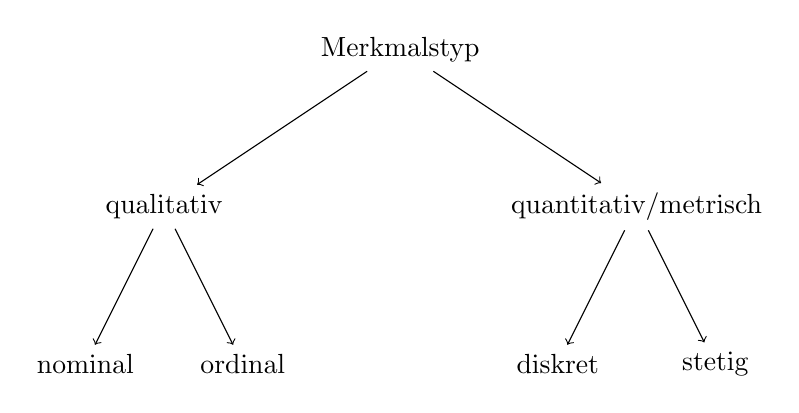
\begin{tikzpicture}
            \node[anchor=center] (a) at (0,0) {Merkmalstyp};
            \node[anchor=center] (b) at (-3,-2) {qualitativ};
            \node[anchor=center] (c) at (3,-2) {quantitativ/metrisch};
            \node[anchor=center] (d) at (-4,-4) {nominal};
            \node[anchor=center] (e) at (-2,-4) {ordinal};
            \node[anchor=center] (f) at (2,-4) {diskret};
            \node[anchor=center] (g) at (4,-4) {stetig};
            \draw[->] (a) -- (b);
            \draw[->] (a) -- (c);
            \draw[->] (b) -- (d);
            \draw[->] (b) -- (e);
            \draw[->] (c) -- (f);
            \draw[->] (c) -- (g);
        \end{tikzpicture}
    \end{center}
\end{document}
